\documentclass[12pt, a4paper]{article}
\usepackage[utf8]{inputenc}
\usepackage{indentfirst}
\usepackage[margin=10pt,labelfont=bf]{caption}
\usepackage[left=3cm,right=3cm,top=3cm,bottom=3cm]{geometry}
\usepackage{titlesec}
\usepackage{enumitem}
\titleformat*{\section}{\bfseries\large}
\titleformat*{\subsection}{\bfseries\normalsize}
\usepackage{graphicx}

\begin{document}

	\begin{center}
	\textbf{\LARGE{Biblioteca de funções para processamento e análise de imagens SAR integrando recursos disponíveis no R}}\\
	\vspace{7mm}
	\textbf{\large{LaCCAN - Laboratório de computação científica e análise numérica}}\\ 
	\vspace{4mm}
	\textbf{\large{Aluno: John Victor}}\\
	\vspace{4mm}
	\textbf{\large{Orientador: Alejandro Frery}}\\
	\end{center}	
        
    \vspace{4mm}
    \section*{\centering{Resumo}}
    \vspace{4mm}
    
Esta apresentação tem como objetivo principal mostrar os avanços feitos com a revisão bibliográfica. Além disso, mostrar uma visão geral sobre o projeto de pesquisa e os assuntos que são necessários para uma boa compreensão da pergunta científica.

	\section{Etapas do seminário}
    
    \begin{itemize}
		\item Imagem Digital
		\begin{itemize}
			\item Definição e representação
            \item Amostragem e quantização
    		\item Imagem multi-dimensional e multi-espectral 
		\end{itemize}
		\item Sensoriamento remoto
			\begin{itemize}
				\item Sensor passivo e Sensor ativo
				\item Espectro eletromagnético e quantização de propriedades físicas
            \end{itemize}
        \item Imagens SAR (Synthetic Aperture Radar)    
            \begin{itemize}
				\item Obtenção de dados
                \item Diferença entre imagens ópticas e imagens SAR
                \item Formato das imagens SAR
			\end{itemize}
		

	\end{itemize}
	
    Sendo assim, uma rápida introdução será mostrada sobre os tópicos listados acima.
    
    \newpage
    
    \section{Imagem Digital}
    	
        \subsection{Definição e representação}
        
    \begin{figure}[!htb]
    	\centering
    	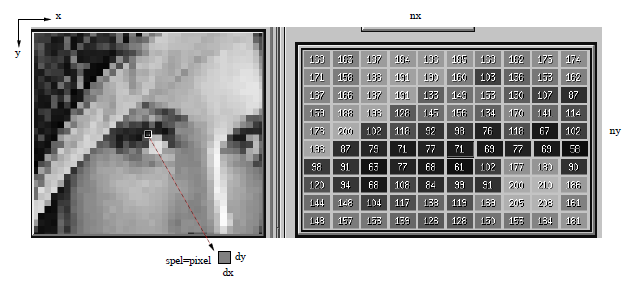
\includegraphics{Screenshot_1}
    	\caption{ cinza (n = 2 e k = 1)}
    	\label{figRotulo}
  	\end{figure}
     \vspace{3mm}
     A imagem digital acima pode ser definida como uma função $\mathbf{f(x,y)}$, tal que o valor gerado pela função representa uma intensidade que varia de $\mathbf{[0, 2^b-1]}$ sendo b o valor de bits por pixel. Além disso, fica fácil perceber que podemos representar essa imagem através de matrizes.
     
    	\subsection{Amostragem e Quantização}
       	
    	\begin{figure}[!htb]
			\begin{center}
				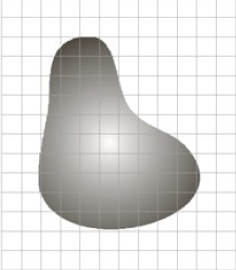
\includegraphics[height=5cm]{Screenshot_2} \quad
				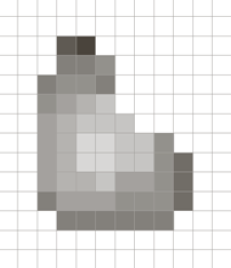
\includegraphics[height=5cm]{Screenshot_3}
			\caption{(1)Matriz de sensores (2)Amostragem e Quantização} 	\label{gdimotes}
			\end{center}
		\end{figure}
    
    A primeira representação é uma imagem continua projetada em uma matriz de sensores, a segunda é o resultado dos processos de Amostragem e Quantização, os quais são responsáveis por transformar valores contínuos em discretos.
    \newpage
    
    \subsection{Imagem multi-dimensional e multi-espectral}
    \vspace{2mm}	
    
    \begin{figure}[!htb]
    	\centering
    	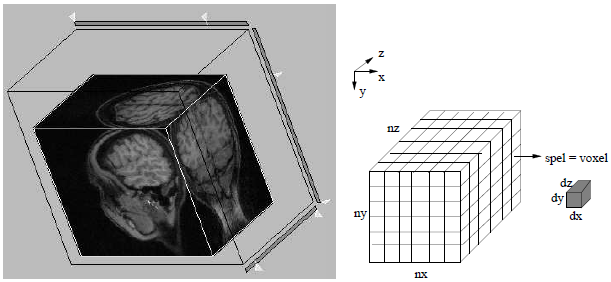
\includegraphics{Screenshot_4}
    	\caption{Imagem de ressonância da cabeça (n = 3 e k = 1)}
    	\label{figRotulo}
  	\end{figure}
    \vspace{3mm}
    Vamos expandir nosso conceito de imagem digital, para imagens que possuem \textbf{n} dimensões e representam \textbf{k} propriedades físicas. Desta forma, podemos obter diferentes propriedades físicas para cada spel combinando bandas espectrais diferentes. 
    % % % ACF O que é "spel"? A frase se repete.
    Logo, uma imagem digital pode ser vista como um par $\mathbf{I'= (D_I, I'')}
$, onde $\mathbf{D_I \subset Z^n\quad\mbox{e}\quad I''(p)=(I_1(p),I_2(p),\dots,I_k(p))}$ é um mapeamento vetorial que associa \textbf{k} valores
inteiros para cada spel $\mathbf{p \in D_I}$.
    
    \section{Sensoriamento Remoto}
    \subsection{Sensor passivo e sensor ativo}
    	\vspace{2mm}
    	\begin{figure}[!htb]
			\begin{center}
				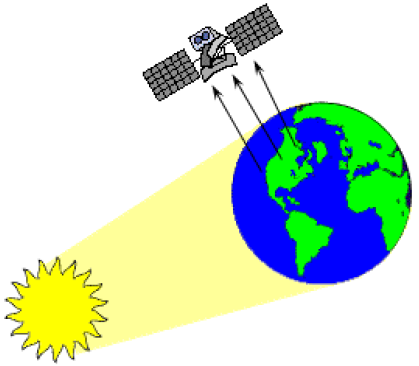
\includegraphics[height=5cm]{Screenshot_5} \quad
				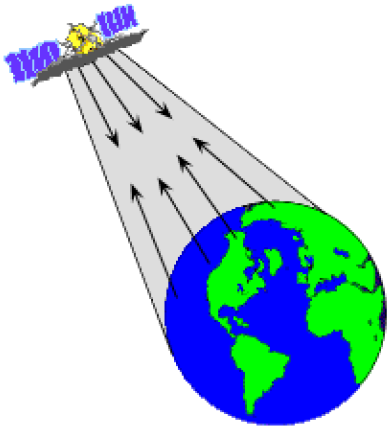
\includegraphics[height=5cm]{Screenshot_6}
			\caption{(1)Sensor passivo (2)Sensor ativo} 	\label{gdimotes}
			\end{center}
		\end{figure}
    
    Sensores ativos captam a energia refletida ou emitida de um alvo que foi iluminado por uma fonte de radiação externa, geralmente o sol. Sensores ativos enviam suas próprias ondas (comprimento longo) para que em seguida possa capta-las, portanto podem monitorar sem a luz do sol e quase não são afetados por condições do tempo.
    \vspace{4mm}
    \subsection{Espectro eletromagnético e quantização de propriedades físicas}
    \vspace{4mm}
    \begin{figure}[!htb]
    	\centering
    	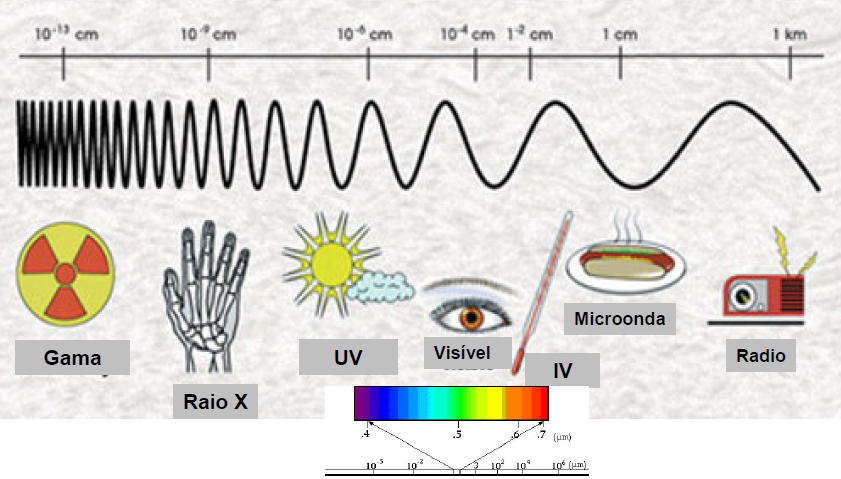
\includegraphics[height = 8cm]{Screenshot_7}
    	\caption{Espectro eletromagnético}
    	\label{figRotulo}
  	\end{figure}
    \vspace{4mm}
    O espectro eletromagnético é a distribuição das ondas eletromagnéticas, visíveis e não visíveis, de acordo com a frequência e o comprimento de onda característico de cada radiação. Podemos combinar diversas bandas espectrais para obter diferentes tipos de informações em cada spel.
    
    \newpage
    \section{Imagens Sar (Synthetic Aperture Radar)}
    \subsection{Obtenção de dados}
    
    \begin{figure}[!htb]
    	\centering
    	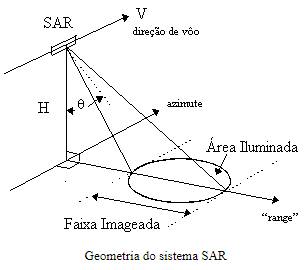
\includegraphics[height = 8cm]{Screenshot_9}
    	\caption{Geometria de imageamento SAR}
    	\label{figRotulo}
  	\end{figure}
    
    A geometria básica de um sistema de imageamento por Radar de Abertura Sintética é mostrado acima. Nesse sistema, a plataforma (avião ou satélite) com o sensor SAR(ativo) se desloca a uma velocidade V em relação ao solo, a uma altura H, apontando a antena lateralmente com um ângulo $\mathbf{\theta}$ em relação ao ponto mais baixo. Durante o percurso vários pulsos são emitidos para que depois sejam captados e processados para gerar uma imagem SAR.
    
    \newpage
    
    \subsection{Diferenças entre imagens opticas e imagens SAR}
    \begin{figure}[!htb]
    	\centering
    	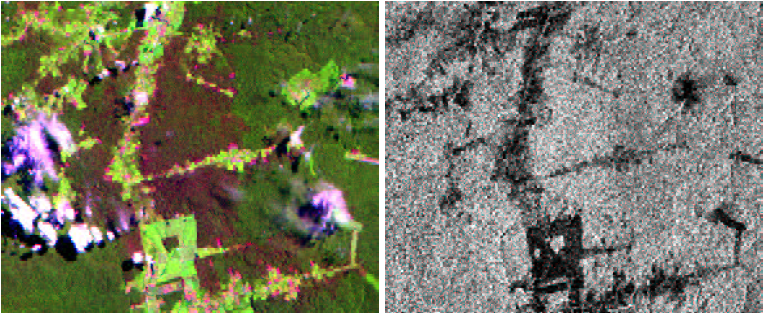
\includegraphics[height = 6cm]{Screenshot_8}
    	\caption{(1)imagem optica (2)imagem Sar}
    	\label{figRotulo}
  	\end{figure}
    
    Como as imagens SAR utilizam a banda espectral das microondas elas podem penetrar determinados alvos, tal penetração depende proporcionalmente do seu tamanho de onda, fica claro perceber que esse sistema de obtenção de imagens é util para obtenção de dados em locais que costumam ter muita interferência climática (Formação de nuvens). Podem perceber que na primeira imagem perdemos as informações que existem abaixo das nuvens, mas isso não ocorre na segunda imagem. 
    \vspace{7mm}
    \section{Considerações finais}
    Logo, foram mostrados algumas definições, representações e conceitos que permeiam a área referente a processamento de imagens em especial SAR, tal revisão ampliou meu entendimento sobre a pergunta de pesquisa. Os próximos passos serão dados em direção a implementação de funções e representações de imagens SAR. 
    
\end{document}